\documentclass[12pt]{article}
\setlength{\oddsidemargin}{0in}
\setlength{\evensidemargin}{0in}
\setlength{\textwidth}{6.5in}
\setlength{\parindent}{0in}
\setlength{\parskip}{\baselineskip}

\usepackage{amsmath,amsfonts,amssymb,graphicx,enumerate,float}

\begin{document}

CSCI 5454 \hfill Problem Set 3\\
Robert Werthman\\
No Collaborators\\

\hrulefill

\begin{enumerate}
	\item
		\begin{enumerate}
			\item \textit{Use the subroutine probefluxcapacitor() to implement the routine randbit() that outputs a uniformly random bit.}\\
			
			\textbf{Pseudocode}
			\begin{verbatim}
			def randbit():
			  while true:
			    (bitA, p) = probefluxcapacitor()
			    (bitB, p) = probefluxcapacitor()
			    if bitA does not equal bitB:
			      return bitA
			
			\end{verbatim}
			
			\textbf{Correctness}\\
			\\
			If the bits were uniformly random then a $1$ or a $0$ would be equally probable.  
			This would mean that the probability that either one would occur would need to be $\frac{1}{2}$ in order to be uniformly random.\\
			\\
			For the problem we are given that $P(1) = p$ and $P(0) = (1-p)$.  
			The first thing we have to figure out is how do we make an algorithm such that the probability of returning a 1 is equal 
			to the probability of returning a 0.  The second thing we have to figure out is how do we make sure the final probability for any run of randbit() is equal $\frac{1}{2}$.\\
			\\
			Notice the probability of two independent events, $A$ and $B$, occurring together is $P(A \cap B) = P(A) \cdot P(B)$ \cite{1}.
			If we let those two events be the probability of randbit() returning a 1, $P(1)$, and the probability of randbit() returning a 0, $P(0)$, 
			then we can say that the probability of them both occurring, $P(1 \cap 0)$, is $p \cdot (1-p)$.  
			This helps because we know that one call to probefluxcapacitor() will either return $p$, for bit value 1, or $(1-p)$, for bit value 0.  
			But if we combine two calls to probefluxcapacitor() sequentially and then compare the results we can create a probability like $P(1 \cap 0)$.\\
			\\
			Two calls to probefluxcapacitor() could result in 4 four combinations:
			\begin{itemize}
				\item $P(1 \cap 1) = p \cdot p$\\
				\item $P(0 \cap 0) = (1-p) \cdot (1-p)$\\
				\item $P(1 \cap 0) = p \cdot (1-p)$\\
				\item $P(0 \cap 1) = (1-p) \cdot p$\\
			\end{itemize}
			The pseudocode above only returns a bit if the probability combination was $p \cdot (1-p)$ or $(1-p) \cdot p$ which are in fact equal to each other.
			This tells us that returning a 1 --- bitA is 1 and bitB is 0 --- and returning a 0 --- bitA is 0 and bitB is 1 --- have equal probability now.  
			And since the if statement only looks at two possible combinations from the two calls to probefluxcapacitor() 
			and out of only one of those possible combinations will a 1 be returned, the probability of returning a 1, $P(1)$, is $\frac{1}{2}$.\\

			\textbf{Runtime}\\
			\\
			In order to find the running time of a randomize algorithm, we need to look at the expectation of the running time.
			The two calls to probefluxcapacitor() each take $O(1)$ because they are just looking at at most two numbers. 
			The checking of the two bits in the if statement is also $O(1)$.  
			This means that one time through the loop takes $O(1)$.
			The probability of getting out of the while loop and returning is $p \cdot (1-p)$ for a 1 or $(1-p) \cdot p$ for a 0.\\
			\\
			Let $X$ be the indicator random variable associated with the returning of randbit().  
			$X_1$ means a 1 is returned and $X_0$ means a 0 is returned.  
			This also means $E[X_1] = P(1)$, the probability of 1 being returned, and $E[X_0] = P(0)$, the probability of 0 being returned.
			This gives us
			\begin{align*}
			E[X] &= \sum_{i=0}^{1} E[X_i]\\
			&= E[X_0] + E[X_1]\\
			&= p \cdot (1-p) + (1-p) \cdot p\\
			&= 2p(1-p)\\
			\end{align*}
			This means the running time of randbit() is $O(2p(1-p) \cdot 1) = O(2p(1-p))$.
			
			\item \textit{Implement the algorithm randbit(p) that outputs 
			an independent random bit with P(randbit(p)=1)=p.}\\
			\\
			\textbf{Pseudocode}
			\begin{verbatim}
			def randbit(p):
			  (k, n) = p
			  l = list of bits
			  for i from 1 to n:
			    bit = randbit()
			    append bit to l
			  if 1 in l:
			    return 1
			  else:
			    return 0

			\end{verbatim}
			\textbf{Correctness}\\
			\\
			randbit() will return a 1 with a probability $p$ of $\frac{1}{2}$.  
			We consider putting the independent event $A$ of running randbit() a single time into a collection.  
			Then running randbit() $n$ times would give us a collection of $n$ events/bits.
			Since these events are all independent then the probability of them happening together is 
			\begin{align*}
			&= P(A_1) \cdot P(A_2) \cdot ... \cdot P(A_n)\\
			&= \frac{1}{2} \cdot \frac{1}{2} \cdot ... \cdot \frac{1}{2}\\
			&= \frac{1}{2^n}\\
			\end{align*}
			$k$ is the number of outcomes we want out of the combined runs of randbit().  
			For example, if we want $P(randbit(\frac{3}{4})=1)=\frac{3}{4}$, then we would need look at the combined output of calling randbit() two times because $n=2$.
			This would give us four possible possible outcomes: (0,0), (1,0), (0,1), (1,1).  
			Out of those four possible outcomes there is a 1 contained in three of them.
			This means that if we return a 1 when a 1 is in a possible outcome we get $p = 3/4$.\\
			\\
			In the pseudocode above we generalize this idea by running randbit() $n$ times and 
			keeping a list of the bits that are returned by randbit().  If a 1 exists in the list then we return a 1
			otherwise we return a 0.\\
			\\
			This technique doesn't appear to work for any other example so it is not correct.
			I was unable to figure out a solution to this problem.
			\\	

			\item \textit{Show the correctness and runtime for randbit(p) when p is not of the form $k/2^n$}\\
			\\
			\textbf{Correctness}\\
			\\
			Let's look at the alorithm when $p = 3/4$.
			This means $p = 0.11$ and $i$ will be in the range 0 to 1.
			$d$ is first set to $b_1$ which is a 1.  Then randbit() is called and its output is compared to $d$.
			The probability of randbit() returning a 0 which would end the function is $1/2$.  
			The next time through $d$ is set to $b_2$ which is a 1.  
			Again randbit() is called and its output is compared to $d$ and the function returns if 
			the output of randbit() is not the same as $d$.
			Each time, the probability of the output of randbit() not being equal to $d$ is $1/2$.\\  
			\\ 
			I don't have any answer for proving the correctness of this problem.\\
			\\
			\textbf{Runtime}\\
			\\	
			We are given that getdigit(p,i) runs in $O(i^c)$ time for some $c$.  
			The if statement where the output of randbit() is compared to $d$ has a probability of $1/2$ of being correct
			each time through the loop.  The loop itself could run a maximum total of $i$ times 
			which is equal to the number of digits in the binary representation of $p$.\\
			\\
			We can then say the upper bound on this function is $O(i (i^c + 1/2))$
		\end{enumerate}

        \newpage
		\item \textit{Give a linear time algorithm that determines if an 
		element appears more than $n/2$ times in an array with probability $1-p$ where $p$ is small.}\\
		\\
		\textbf{Pseudocode}
		\begin{verbatim}
		def AppearsOften(A):
		  n = total elements in A
		  counter = 0
		  i = 1
		  if n > 1:
		    for j from 1 to n:
		      if arethesame(i,j):
		        counter = counter + 1
		      elif !arethesame(i,j):
		        counter = counter - 1
		      if counter < 1:
		        if j < n:
		          i = j + 1
		          counter = 0
		    if counter > 0:
		      return 'YES'
		    else:
		      return 'NO'
		  else:
		    return 'YES' # Single element in the array so it must occur > n/2 times
		\end{verbatim}
		\textbf{Correctness}\\
		\\
		The algorithm AppearsOften() goes through all of the elements in array $A$ and attempts to keep a count of the
		element that appears most often in $A$.  The base case, when $i = 1$, occures when $A$ has only one element and the algorithm returns ``YES'' because $n/2 = 1/2$ and the element occures one time which is greater than $1/2$.
		\\
		For the inductive step we assume $n > 1$ and $i,j \le n$.  Each iteration through the loop, we compare the $i$th element with the $j$th element.  If they are the same we increment the counter otherwise we decrement the counter.  The counter helps to determine if after having gone through the elements in the array there is an element $x$ that occurs $> n/2$ times.  The counter would need to be greater than 1 in order for there to be an element that occurs $> n/2$ times.  We can think of this as breaking the array into comparisons between pairs.  $x$ would occur in a lot of pairs because it is the element that occurs the most so the counter would end up being higher after the completion of the for loop.\\
		\\
		This algorithm will return ``NO'' when there isn't an element that occurs $> n/2$ times but it will also return ``NO'' in some cases when there is an element $> n/2$.  This also occurs for ``YES'' so I am unable to prove it correctly says ``NO'' if there is no such element and ``YES'' with probability $1-p$.\\      
		\\
		\textbf{Runtime}\\
		\\
		The algorithm goes all $n$ elements of array $A$ at most one time.  
		Keeping a counter and checking if elements are the 
		same and checked the value of the counter take constant time, O(1), each.
		This means the runtime for this algorithm is $O(n)$.
		
		\newpage
		\item \textit{Help Gru understand his minion dispensing situation}
		\begin{enumerate}
		    \item \textit{What is the expected number of minions in the first pod after t seconds?}\\
		    \\
		    If a minion is added to a pod every second we expect there to be a total of $t$ minions combined from all of the pods after $t$ seconds.   Let $X$ be the random variable that represents the number of minions in the first pod.  After time $t$, $X$ can be between 0 and $t$ which means the pod can contain between 0 and $t$ minions.  The expected value of the number of minions $i$ in the first pod after time $t$ can be represented as the binomial distribution \cite{2}
		    \begin{align*}
		    E[X] &= \sum_{i=1}^{t} i\binom{t}{i}\frac{1}{k^i}(1-\frac{1}{k})^{t-i}\\
		    &=\frac{t}{k}\\
		    \end{align*}
		    \item \textit{In expectation, when will the first pod get its first minion?}\\
		    \\
		    Let $X$ be the random variable that represents the number of minions that are dispensed before a minion goes into the first pod.  The expected value of the number of minions $i$ that are dispensed before the first pod will get a minion can be represented as the geometric distribution \cite{3}
		    \begin{align*}
		    E[X] &= \sum_{i=1}^{\infty} i(1-\frac{1}{k})^{i-1} \cdot \frac{1}{k}\\
		    &= k\\
		    \end{align*}
		    
		    \item \textit{In expectation, when will all pods have at least one minion?}\\
		    \\
		    Let $n$ be the number of minions we need to dispense in order to have at least one minion in all $k$ pods.  Let $n_i$ be the number of minions we have to dispense in order to fill the ith pod.  The probability that the ith pod will be filled is $(k-i+1)/k$.  The expected time until the ith pod gets a minion is $k/(k-i+1)$. The expected value of $n$ is then \cite{4}
		    \begin{align*}
		        E[n] &= \sum_{i=1}^{k} E[n_i]=\sum_{i=1}^{k} k/(k-i+1)\\
		        &\le \sum_{i=1}^{k} k/(k-i)=k\sum_{i=1}^{k} 1/(k-i)\\
		        &\le k\sum_{i=1}^{k} 1/i=\theta(k\,log\,k)\\
		    \end{align*}

		    \item \textit{Plot 3c, $c_1f(k)$, $c_2f(k)$.}\\
		    \\
		    \begin{figure}[H]
		    \centering
			  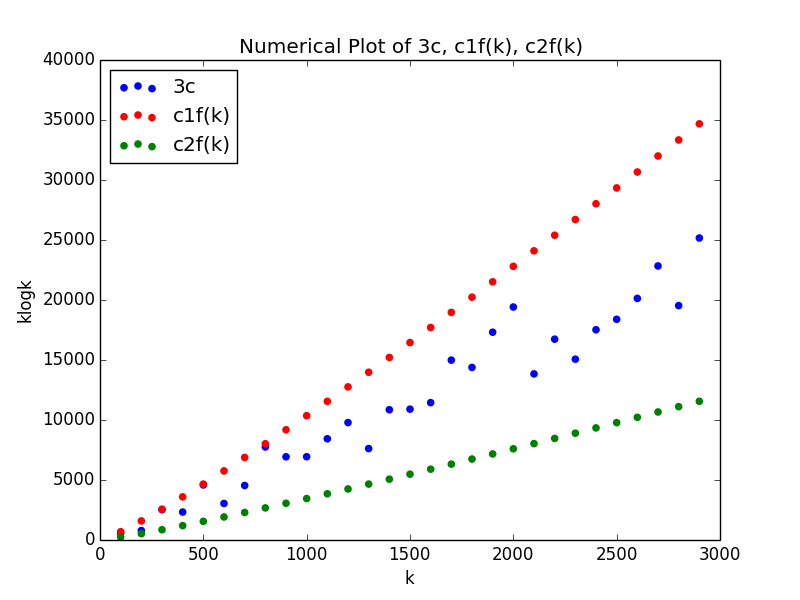
\includegraphics[width=9cm]{q3_3d.png}
			  \end{figure}
		    I let $c_1 = 1.5$ and $c_2 = .5$.
		\end{enumerate}

		\newpage
		\item \textit{Implementation of Karger's min-cut algorithm using Kruskal's algorithm.}
		\begin{enumerate}
			\item \textit{Explain how to view Karger’s algorithm as constructing a spanning tree.}\\
			\\
			A spanning tree is a subgraph that is a tree that includes all of the vertices in the graph \cite{6}.  It won't necessarily include all of the edges in a graph.  Karger's randomly chooses an edge and contracts it making the two vertices at the endpoints of the edge into one vertex.  It then reconnects all of the edges from those two vertices to the now single vertex except the one edge it contracted.  By the end of the algorithm it will have chosen enough edges to contract that all of the vertices in the graph would have been one of the endpoints of a contraction.  Karger's returns a subgraph made up of two vertices of the original graph which can be said to be a spanning tree of the original graph.\\   
			\\
			\item \textit{Show that the probability of spanning tree T being selected is the same in both.}\\
			\\
			When Karger's algorithm chooses a random edge and then contracts it, it almost like running Kruskal's with uniform random weights \cite{5}.  Kruskal's algorithm will choose the minimum weight edge which has the same probability as Karger's choosing a random edge.\\  
			\\
			We can say that in a uniform distribution the probability of choosing an edge is the same for every edge.  In the case of Karger's if we have $k$ edges then in a uniform probability distribution the probability of choosing any edge is $1/k$.  In the case of Kruskal's algorithm, if we have $k$ edges and each with a uniformly random weight choosed the probability of choosing the lowest weight will be $1/k$ assuming there are no duplicate weights.\\
			\\
			Let $X$ be the random variable that the spanning tree $T$ will be selected by Karger's and $Y$ be the random variable that the spanning tree $T$ will be selected by Kruskal's.  For their distributions to be the same \cite{7}
			$$
			P(X \le x) = P(Y \le x) \,\text{for all}\, x
			$$
			This means the moment generating functions for these variables need to be the same in order for the their distributions to be the same.  Since we know both are continous uniform distributions and the probability of selecting an edge is the same, their moment generating funcitons are the same and the probability of selecting $T$ is the same.\\
			\\
			\item \textit{Assuming T was chosen by both algorithms, explain why the max-weight edge of T in Kruskal defines the final cut output by Karger.}\\
			\\
			In Kruskal's the max-weight edge will be the last edge chosen since Kruskal's algorithm chooses edges that are the minimum weight left in the graph.  In Karger's algorithm the final cut is involves the last edge left after all contractions of the graph have taken place.  If the probabilities are uniform for choosing an edge in both algorithm's, the max-weight edge in Kruskal's will be the final cut edge in Karger's since it is the last edge remaining in the graph.\\ 
			\\
			\item \textit{Put the above three steps together to prove the equivalence of the two algorithms: the distribution over cuts they return is the same.}\\
			\\
			Kruskal's algorithm produces a spanning tree and in part (a) we showed that Karger's algorithm also produces a spanning tree.  In part (b) we showed that the probability of selecting a spanning tree is the same.  In part (c) we showed that the last (max-weight) edge chosen by Kruskal's is the same as the edge chosen by Karger's that the min-cut crosses.\\
			\\
			Combining all three parts we can say both produce a spanning tree, both produce the same spanning tree, and if we were to remove the max-weight edge from the spanning tree Kruskal's algorithm produces it would be the same edge that the min-cut crosses in Karger's.  All things being equal, randomized Kruskal's with max-weight edge removal is the same a Karger's min-cut algorithm because they both return the same cut of vertices.\\
		\end{enumerate}

		\newpage
		\item \textit{Implement Karger's min-cut algorithm.}\\
    \begin{enumerate}
    \item \textit{Show the probability of Karger's finding a min cut with different size graphs.}\\
          \begin{figure}[H]
		      \centering
			    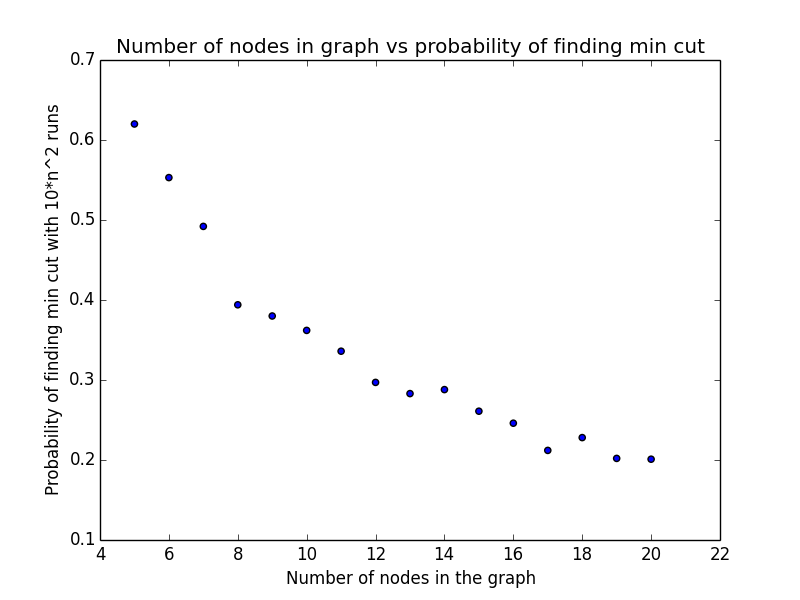
\includegraphics[width=9cm]{q3_5a.png}
			    \end{figure}
    \item
    \end{enumerate}

		\newpage
		\item \textit{Help minion captain A maximize the sum of the player's abilities on his team.}\\
		\\
		\textbf{Pseudocode}
		\begin{verbatim}
		def PlayerSelection(L):
		// L is the line of players organized like an array
		// of size n where L[0] is the front of the line and L[n-1] is the end
		// and those are the abilities of those players

		i = 0
		j = |L| - 1 // j = n - 1

		// This will be a list of the order to choose players
		// Assuming there is an even number of players
		optimal_player_selection[j/2] 

		while True:
		  // Find the max ability when choosing the current first player in line
		  // Look ahead to A's next turn
		  first = max(L[i] + max(L[i+2], L[j]), L[i]+max(L[i+1],L[j-1]))

		  // Find the max ability when choosing the current last player in line
		  // Look ahead to A's next turn
		  last = max(L[j] + max(L[i+1], L[j-1]), L[j]+max(L[i],L[j-2]))

		  // Find the max ability out of choosing the first and last player
		  // By adding the ability of this player plus the next turn's player
		  if max(first, last) == first:
		    // Choose first player in line
		    optimal_player_selection.append(i)
		    i++
		    // B chooses next highest ability player
		    m = max(L[i],L[j])
		    if L[i+1] == m:
		  	  i += 1
		    else:
		      j -= 1
		  else:
		    // Choose last player in line
		    optimal_player_selection.append(j)
		    j--
		    // B chooses next highest ability player
		    m = max(L[i],L[j-1])
		    if L[i] == m:
		  	  i += 1
		    else:
		      j -= 1
		  // If we have two players left then choose the player with the 
		  // highest ability and return the array of players 
		  if i == j-1:
		    m = max(L[i],L[j-1])
		    if L[i] == m:
		  	  optimal_player_selection.append(i)
		    else:
		      optimal_player_selection.append(j)
		    return optimal_player_selection
		\end{verbatim}
		\textbf{Correctness}\\
		\\
		I found that greedily choosing the player at the front or end of the line with the highest ability when it is $A$'s turn does not maximize the sum of the player's abilities on the team.  Neither does trying to minimize the player's abilites that $B$ can choose from when it is $B$'s turn to go after $A$.\\
		\\
		The optimal strategy for this problem is a dynamic programming algorithm.  I assume $B$'s strategy is the greedy approach where the player with the highest ability is chosen from the front or end of the line when it is $B$'s turn.  I could not figure out a way to maximize the sums of the player's ability if $B$ used the same strategy I did.\\
		\\
		The key to my algorithm is to look ahead to $A$'s next move and make the current choice of a player based on maximizing the sum of the current player's ability with the next player's ability that I choose.\\
		Given a line $L$ and it is $A$'s turn to choose a player and there are $j - i$ players, where $j = |L|$, remaining in line, $A$ can either choose the first player in line, $L[i]$, or the last player in line, $L[j]$.  $B$, depending on the choice $A$ makes, will then be able to choose between $L[j], L[i+1], L[j-1], L[i]$.  $B$ will choose the player with the highest ability if $B$ is following the greedy strategy.  This means that we can see what players will be availabe in turn number two for $A$ because we know $B$'s choice for its turn.  We then decide which future player will maximize the sum of the abilities of the the current player with the future player.  Doing this every turn gaurantees that we will maximize the sum of the abilities of all the future players with the current players giving $A$ the maximized sum of player abilites on his final team.\\    
		\\
		\textbf{Runtime}\\
		\\
		If the line of players is size $n$ then this algorithm has a runtime of $O(n)$.  It will loop through the line of players until there are only two players left.

		\newpage
		\item \textit{Describe the probability that Gru can launch...}
		\begin{enumerate}
			\item \textit{With a recursive formulation that expresses the problem in terms of smaller verions of the problem.}\\
			\\
			The first minion has a probability of $1/n$ of standing in his correct position because he chooses randomly.  The probability of a minion that doesn't choose randomly standing in his correct position is 1.  He will always stand in his correct position.\\
			\\  
			We define $P(i)$ as the probability of the ith minion being in its correct position. We define $y_i=0$ if the position of the ith minion is not occupied and $y_i=1$ if the position is occupied.  Since the probability of a minion being in its correct position depends on the minions before it being in their correct positions we can define the recursive formula of the probabilty of a minion being in its correct position as 
			$$
			P(i) =
			\begin{cases}
			1/n & \quad \text{if } i = 1\\
			P(i-1) \cdot 1 & \quad \text{if } i > 1 \text{ and } y==0\\
			P(i-1) \cdot 1/n & \quad \text{if } i > 1 \text{ and } y==1\\
			\end{cases}
			$$
			The probability of Gru lauching is the probability of the last minion being in its correct position which is the probability $P(n)$ defined by the recursive formula above.

			\item \textit{Without a recurrence in a short paragraph.}\\
			\\
			Because the first minion chooses his position randomly the first minion has a probability of $1/n$ of choosing the correct position.  If he does then all of the other minions will be in their correct positions including the final minion and Gru will lauch with a probability of $1/n$.\\
			\\
			If the first minion does not choose his correct postion then we can assume that at least a second minion will a choose a position randomly.  This shows that the probability of a minion choosing his correct position depends on the probability of previous minions choosing their correct position.  If a minion's position is occupied then he will choose someone else's position.  A minion choosing his position is a dependent event so the probabilities of each minion choosing his position is mulitplied.\\
			\\
			Gru's probability of lauching is the probability of the last minion $n$ being in his correct position which is the product of the probabilities of all of the other minions being in their correct positions.
		\end{enumerate}

\end{enumerate}

\newpage
\begin{thebibliography}{10}
	\bibitem{1} https://www.mathsisfun.com/data/probability-events-independent.html
	\bibitem{2} https://en.wikipedia.org/wiki/Binomial\_distribution
	\bibitem{3} https://en.wikipedia.org/wiki/Geometric\_distribution
    \bibitem{4} http://tuvalu.santafe.edu/~aaronc/courses/5454/csci5454\_spring2013\_L4.pdf
    \bibitem{5} https://en.wikipedia.org/wiki/Karger\%27s\_algorithm
    \bibitem{6} https://en.wikipedia.org/wiki/Spanning\_tree
    \bibitem{7} https://en.wikipedia.org/wiki/Random\_variable\#Equality\_in\_distribution
\end{thebibliography}

\end{document}
